%----------------------------------------------------------------------------
\documentclass{article}
%----------------------------------------------------------------------------
\usepackage[a4paper, top=20mm, bottom=20mm, left=20mm, right=20mm]{geometry}
%----------------------------------------------------------------------------
\usepackage{paracol}
\usepackage{graphicx}
\usepackage{hyperref}
\usepackage[dvipsnames]{xcolor}
\usepackage{lipsum}
\usepackage{fancyhdr}
\usepackage[ngerman]{babel}
\usepackage{csquotes}
\usepackage{float}
%----------------------------------------------------------------------------
\graphicspath{ {./images/} }
%----------------------------------------------------------------------------
% fancyhdr setup
%----------------------------------------------------------------------------
\pagestyle{fancy}	% activate fancy style
\fancyhf{}			% clear fancy settings
% Header
\fancyhead[L]{Meilenstein 1}
\fancyhead[R]{v1.0}
% Footer
\fancyfoot[C]{Seite \thepage}
\fancyfoot[R]{\today}
% lines
\renewcommand{\headrulewidth}{0.4pt}
\renewcommand{\footrulewidth}{0.4pt}
%----------------------------------------------------------------------------
% first page setup
%----------------------------------------------------------------------------
\title{Teamprojekt}
\author{Leonidas, Vincent, Nicko, Alexander Grath}
\date{} % empty date
%----------------------------------------------------------------------------
% reference definitions
% to use references: compile with bibtex then with pdflatex
%----------------------------------------------------------------------------
\begin{filecontents}{references.bib}
@article{doe2023,
  author  = {Doe, John and Smith, Jane},
  title   = {An Analysis of Citation Styles},
  journal = {IEEE Transactions on Automatic Formatting},
  volume  = {10},
  number  = {2},
  pages   = {100--105},
  year    = {2023}
}
%
@book{knuth1984,
  author    = {Knuth, Donald E.},
  title     = {The TeXbook},
  publisher = {Addison-Wesley},
  year      = {1984}
}
\end{filecontents}
%############################################################################
\begin{document}
%
\maketitle
%
\thispagestyle{empty} % clear page number
%
% sub-title of the document
\begin{center}
\section*{M1 Problemanalyse}
\end{center}

% universität wien logo
\begin{figure}
	\centering
	
\includegraphics[scale=.6]{univie}
\end{figure}
%
\newpage
%
\tableofcontents
%
\setcounter{page}{1} % restart page count at 1
%
\newpage
%
% The \inputs can be change to \include if needed
% put your section in the section folder and only change this document by adding another \input{...}
% the sections are <name>_<chapter>.tex files and do NOT include any document structure code
% thre is nothing fancy going on, the content of the files is just pasted here:
%
\section{Leonidas}
\lipsum[1-3]

\section{Vincent}
\lipsum[1-3]

\section{Nicko}
\lipsum[1-3]

\section{Alexander}
\lipsum[1-3]

%
\section{Analyse von vorhandener Literatur}
\lipsum[1-2]
%
\section{Analyse von Konkurrenzprodukten}

\subsection{Marktüberblick}

Eine erste Orientierung liefert das Anwendungsverzeichnis von \texttt{data.gv.at} für den Publisher \enquote{Stadt Wien}. Auf den ersten Blick erscheint das Angebot mit insgesamt $n = 345$ Anwendungen sehr umfangreich. Diese Zahl relativiert sich jedoch deutlich, sobald nur jene Anwendungen betrachtet werden \url{https://www.data.gv.at/applications?locale=de&page=1&publisher=Stadt+Wien}, die offene Daten tatsächlich visualisieren. Unter dieser Einschränkung reduziert sich das Feld auf rund $n = 100$ Anwendungen. Wird zusätzlich nach Webanwendungen gefiltert, verbleiben $n = 36$ Angebote und bei mobilen Anwendungen sind es nur noch $n = 8$.

Für die vorliegende Arbeit ist insbesondere diese letzte Gruppe relevant, da sich das Projekt auf eine mobile App bezieht. Die nähere Betrachtung zeigt jedoch, dass es sich dabei überwiegend um hoch spezialisierte Anwendungen oder um ältere, teilweise wahrscheinlich nicht mehr aktiv genutzte Angebote handelt. Diese Lösungen sind in ihrer Zielsetzung und im Nutzungskontext nur eingeschränkt mit dem hier verfolgten Konzept einer allgemeinen Open-Data-Visualisierung vergleichbar. Daraus lässt sich ableiten, dass im spezifischen Umfeld der Wiener Open Data nur eine geringe direkte Konkurrenz besteht. Insbesondere für mobile Anwendungen im Bereich allgemeiner Open-Data-Visualisierung ist derzeit kaum ein unmittelbar vergleichbares Produkt vorhanden.

\subsection{Vergleich geeigneter Referenzplattformen}

Da im mobilen Bereich kaum tragfähige Vergleichsprodukte existieren, werden im Folgenden webbasierte Anwendungen als Referenzplattformen herangezogen. Diese Anwendungen sind zwar keine direkten mobilen Konkurrenzprodukte, zeigen jedoch etablierte Gestaltungs- und Interaktionsmuster für die Exploration, Filterung und Visualisierung offener Daten. Besonders relevant sind dabei thematische Navigation, interaktive Diagramme, Kartenansichten, Vergleichsfunktionen sowie die verständliche Aufbereitung komplexer Datensätze.

\subsubsection{Winterthur in Zahlen}
Winterthur in Zahlen ist ein interaktives städtisches Dashboard der Stadt Winterthur. Es zeigt aktuelle Daten rund um die Stadt und ist in den Bereich Statistik und Daten der Stadt eingebettet. Auff\"allig leicht ist die Bedienung der Seite man w\"ahlt ein Thema aus siehe  Bild 
\ref{fig:winterthur-start} und dann bekommt man automatisch Statistiken und Visualisierungen bereitgestellt.

\begin{figure}[H]
    \centering
    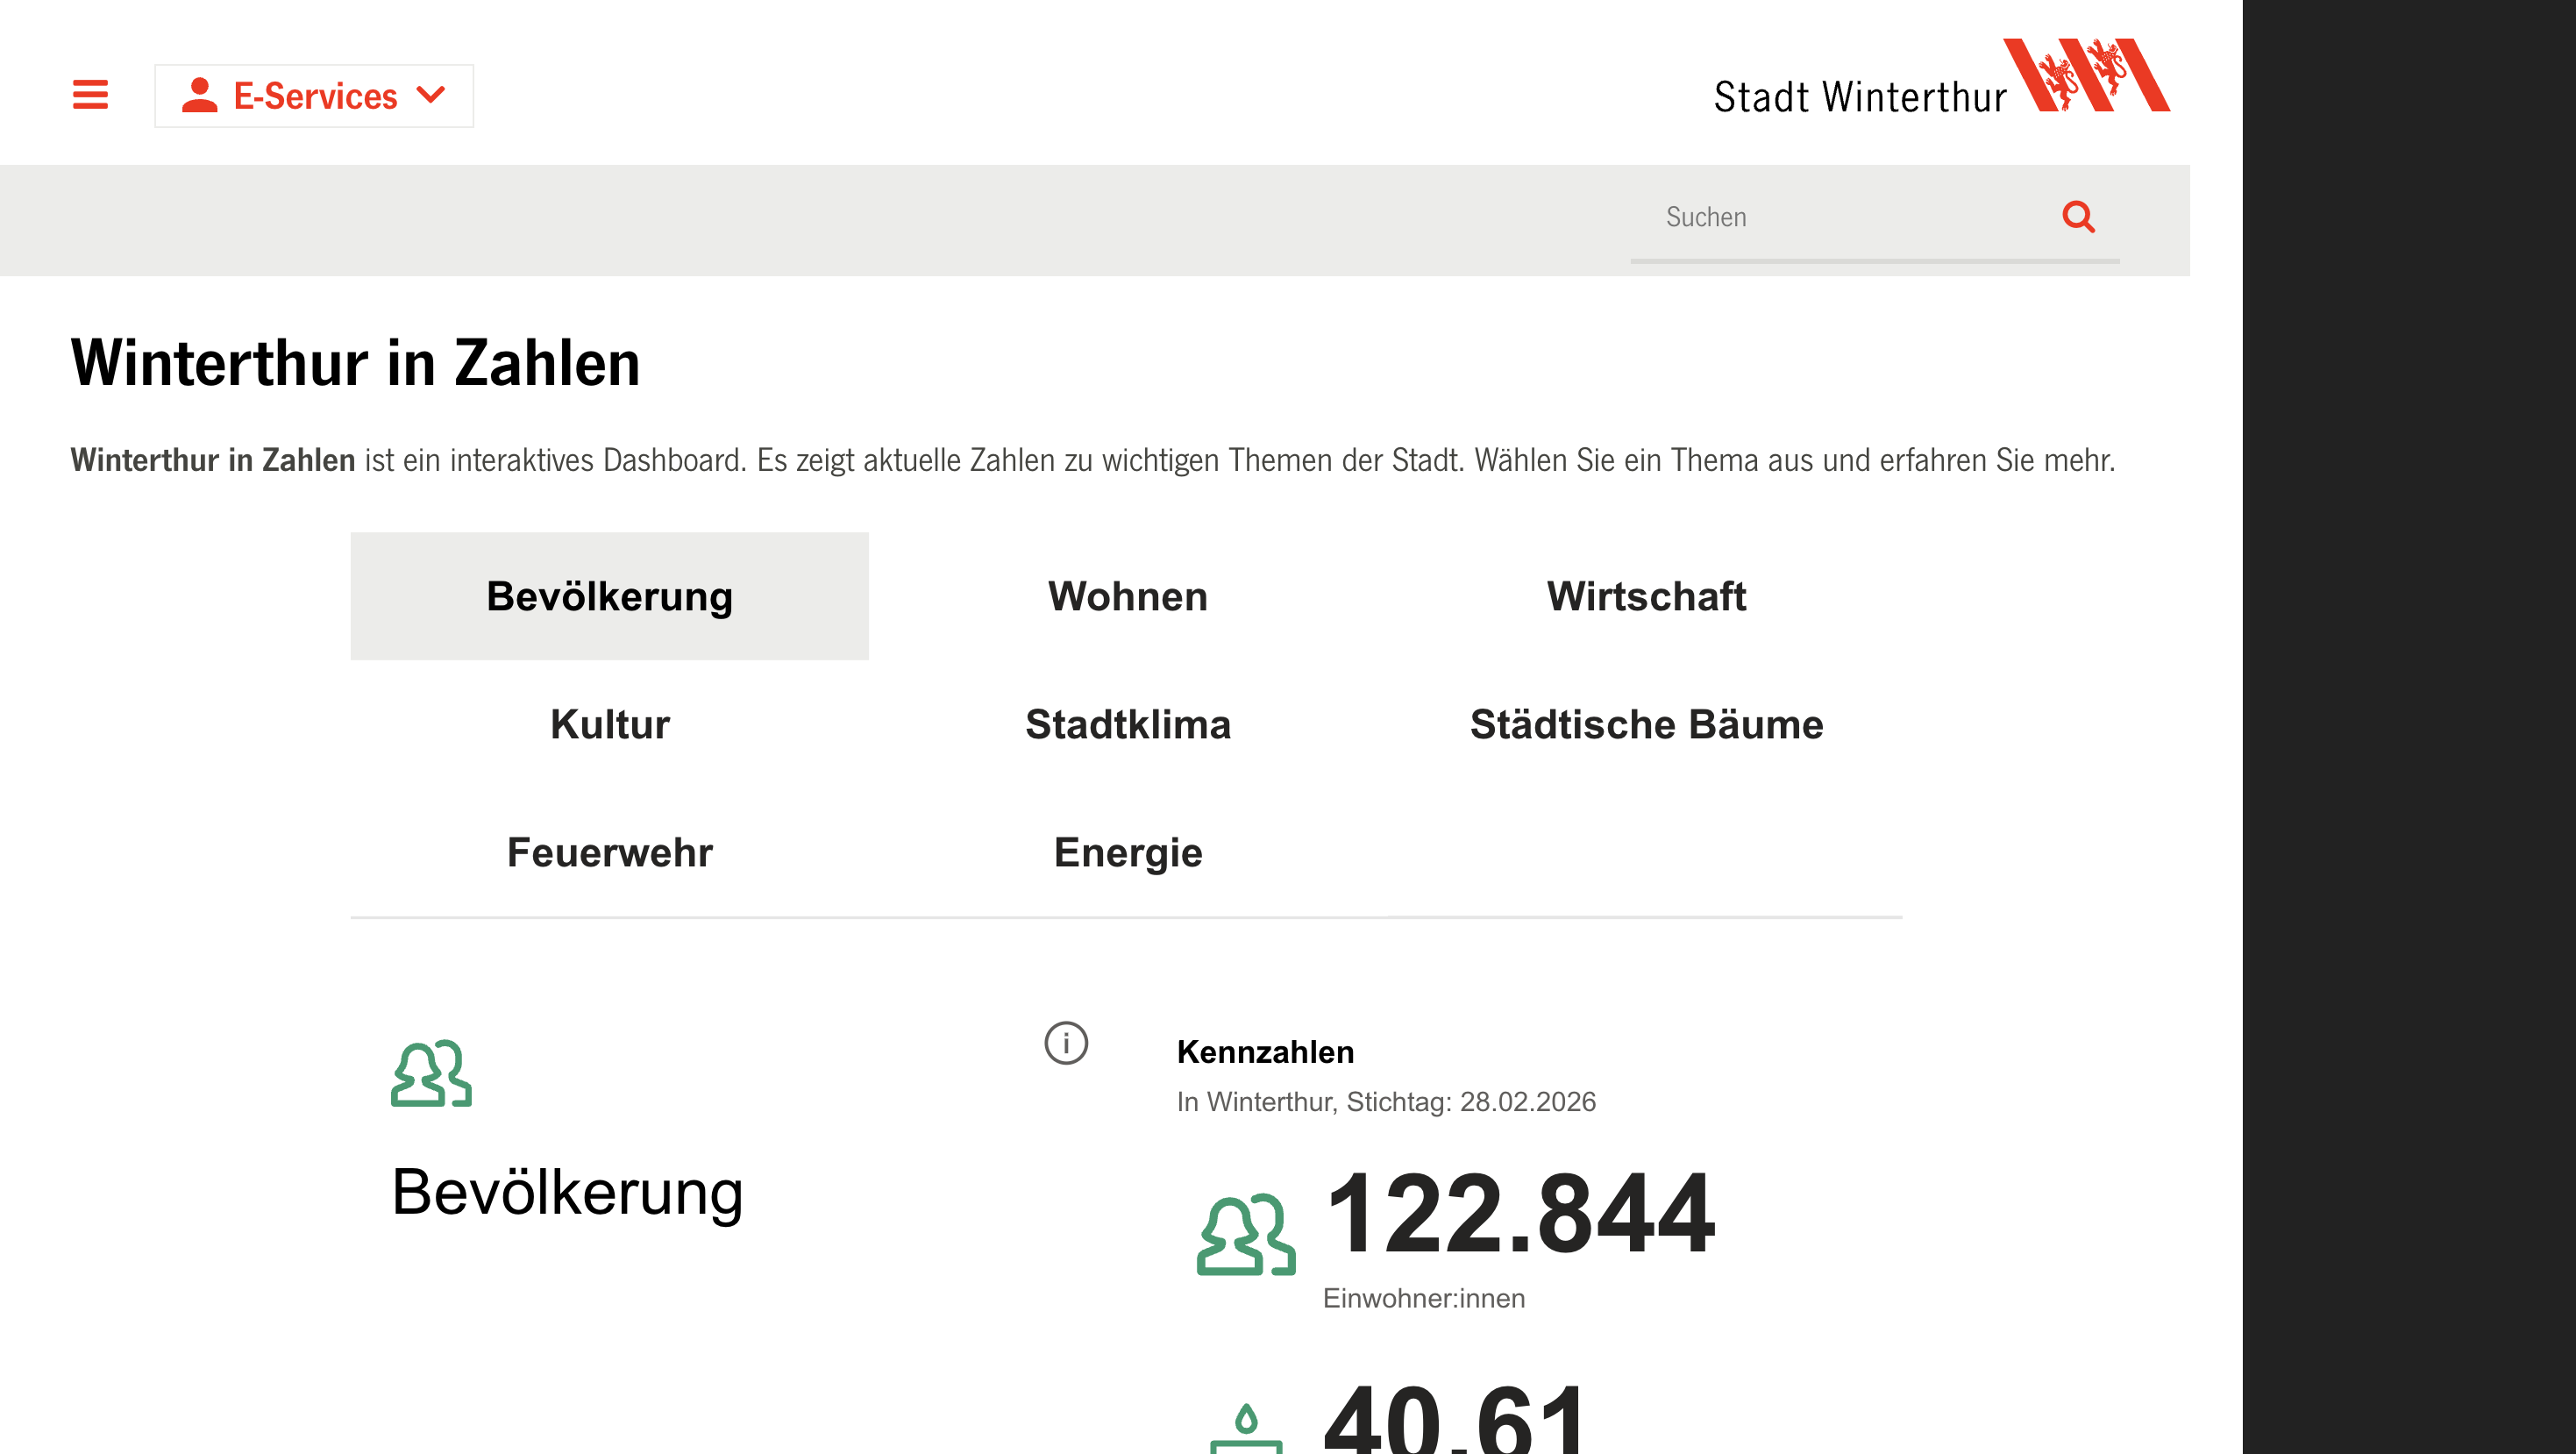
\includegraphics[width=0.90\textwidth]{../images/StadtWinterthur.png}
    \caption{Startseite von \emph{Winterthur in Zahlen}. Die Plattform bietet einen thematisch strukturierten Einstieg in städtische Kennzahlen.}
    \label{fig:winterthur-start}
\end{figure}

Die Startseite zeigt eine klar strukturierte thematische Navigation, über die unterschiedliche Themenbereiche direkt angewählt werden können. Dieses Muster ist für eine mobile Open-Data-Anwendung besonders relevant, da es einen einfachen und intuitiven Zugang zu komplexen Datensammlungen ermöglicht.

\begin{figure}[H]
    \centering
    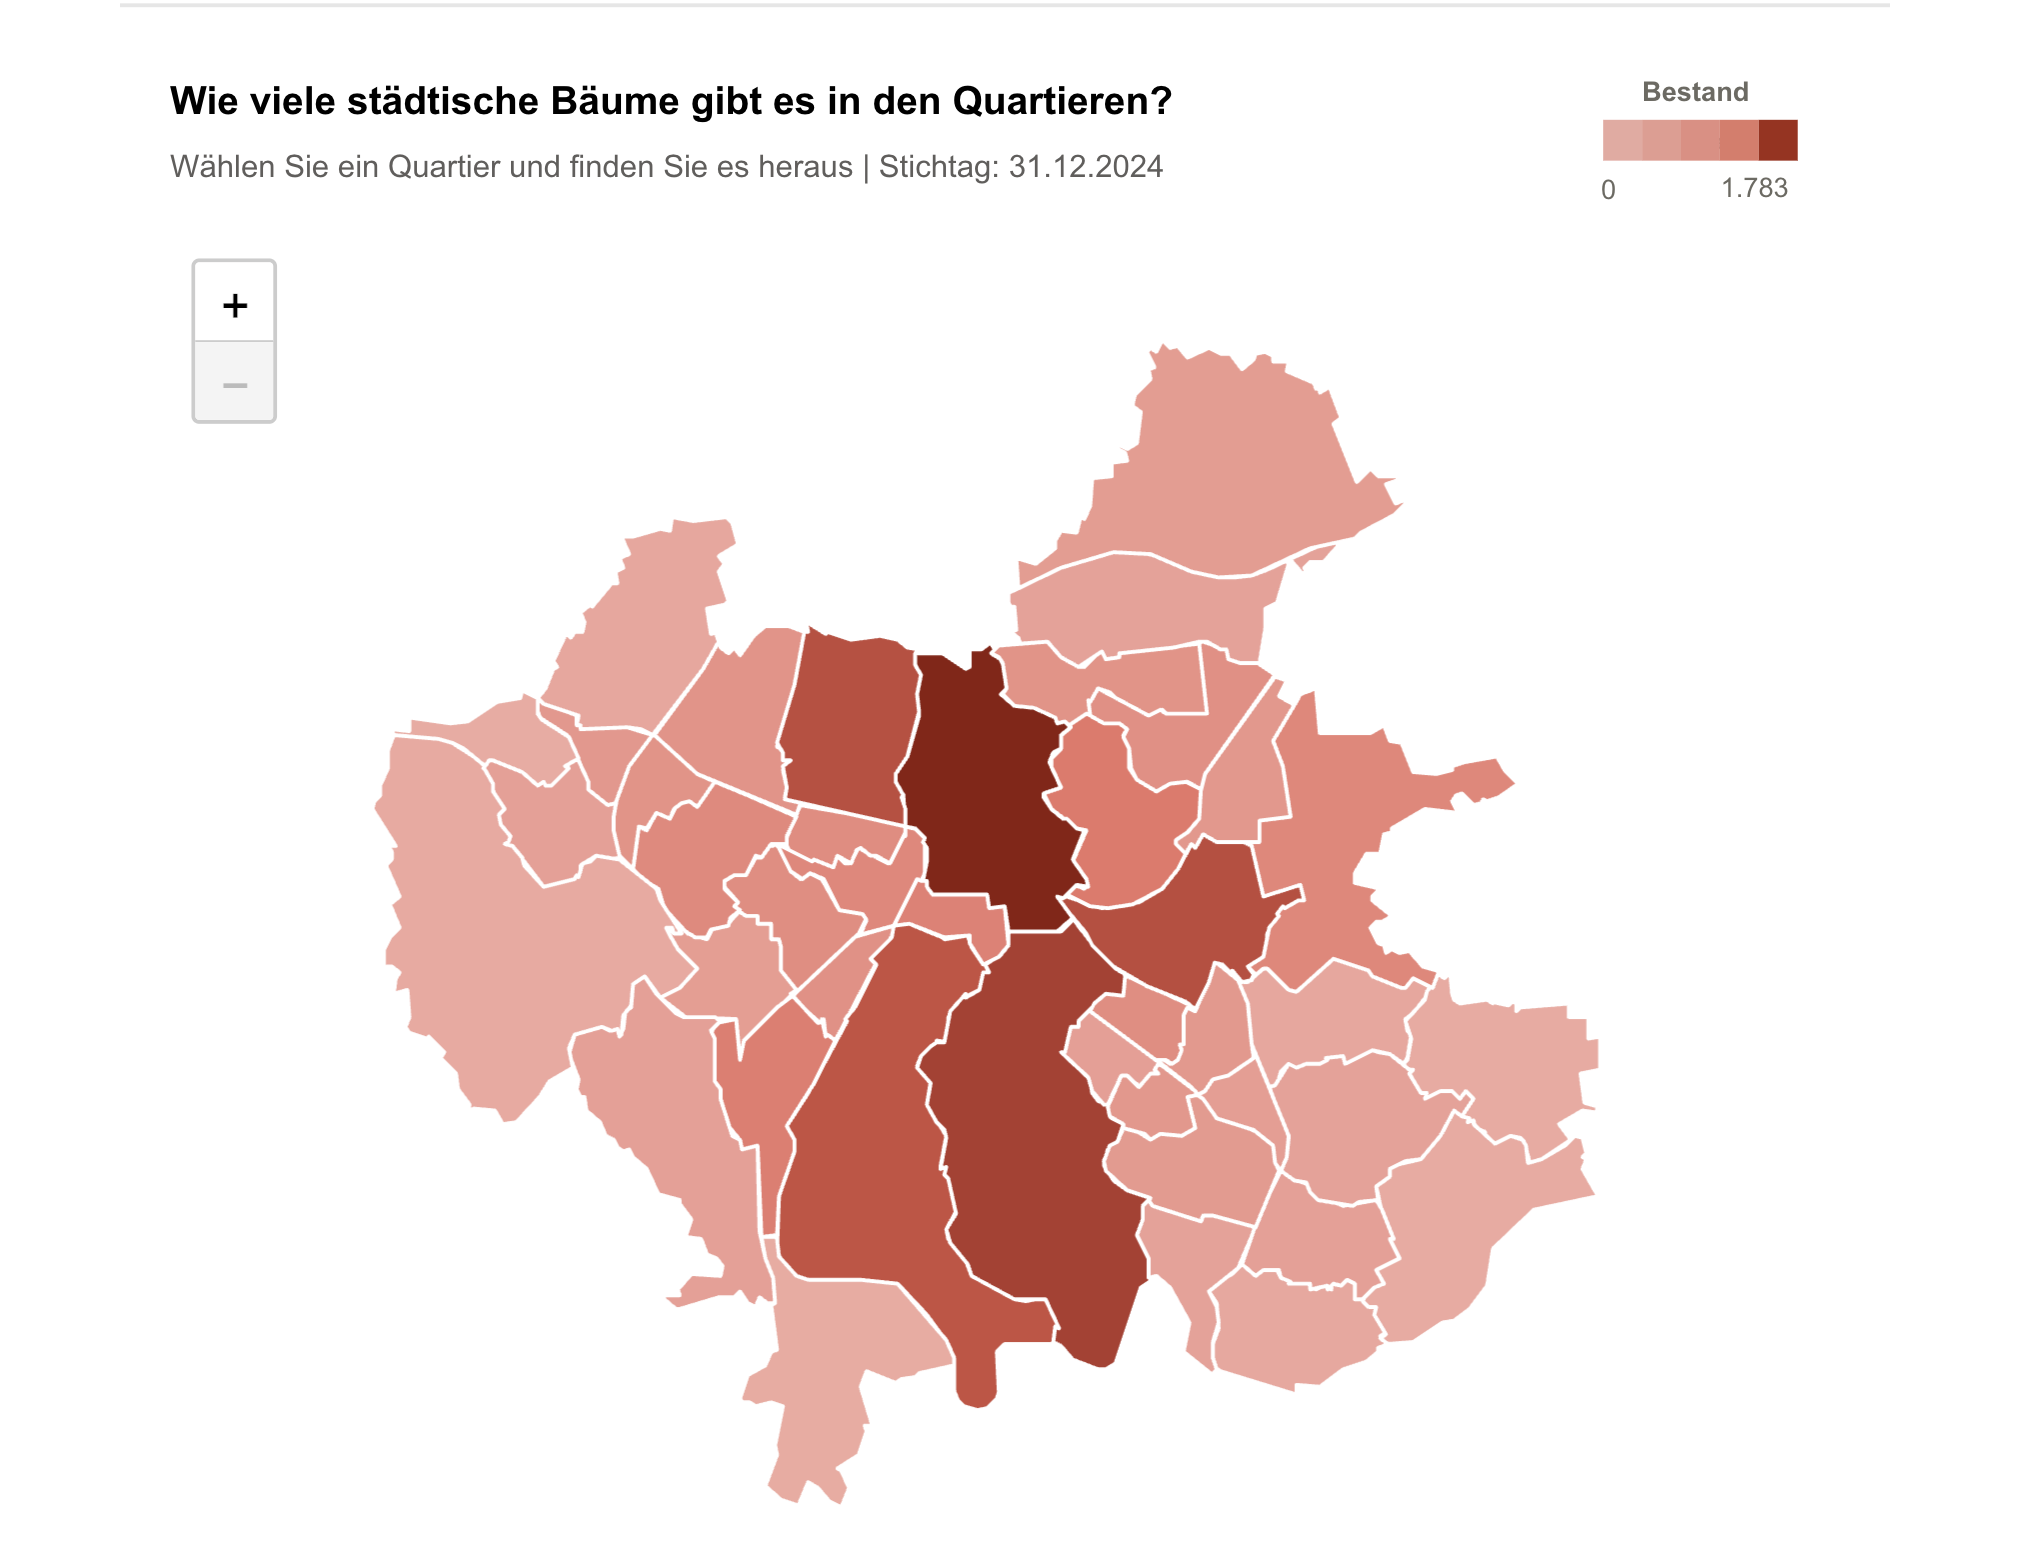
\includegraphics[width=0.82\textwidth]{../images/StadtWinterthur_vis.png}
    \caption{Kartenbasierte Detailansicht innerhalb von \emph{Winterthur in Zahlen}. Die Plattform kombiniert thematische Orientierung mit visueller Exploration.}
    \label{fig:winterthur-detail}
\end{figure}

\begin{enumerate}
    \item \textbf{Vorteile}
    \begin{enumerate}
        \item Die Plattform weist eine sehr flüssige und reaktionsschnelle Bedienung auf.
    \end{enumerate}

    \item \textbf{Nachteile}
    \begin{enumerate}
        \item Die Plattform bietet nur geringe Möglichkeiten zur individuellen Anpassung der Darstellung.
        \item Auf der Startseite bleibt am rechten Rand eine ungenutzte dunkle Fläche sichtbar, wodurch der verfügbare Platz nicht vollständig ausgeschöpft wird.
    \end{enumerate}
\end{enumerate}


\subsubsection{visualize.admin.ch}
Die Plattform ermöglicht die Visualisierung von Schweizer Open-Data-Datensätzen und bietet dabei zahlreiche Anpassungsmöglichkeiten. Gleichzeitig ist ihre Bedienung jedoch vergleichsweise anspruchsvoll, da nicht vorgegeben wird, welche Darstellungen sinnvoll sind. Stattdessen müssen die Nutzerinnen und Nutzer selbst entscheiden, welche Daten wie visualisiert werden sollen. Dadurch besteht ein erhöhtes Risiko für Fehlinterpretationen oder Missbrauch. Gerade für Laien kann es schwierig sein zu erkennen, welche Darstellungsformen sich für eine fundierte und aussagekräftige Analyse am besten eignen. Vgl. \url{https://visualize.admin.ch/?dataSource=Prod}
\begin{figure}[H]
    \centering
    \begin{minipage}[t]{0.48\textwidth}
        \centering
        
\includegraphics[width=\linewidth]{../images/SwissOpenGov.png}
        \vspace{0.4em}

        \small (a) Startseite von \emph{visualize.admin.ch}
    \end{minipage}
    \hfill
    \begin{minipage}[t]{0.48\textwidth}
        \centering
        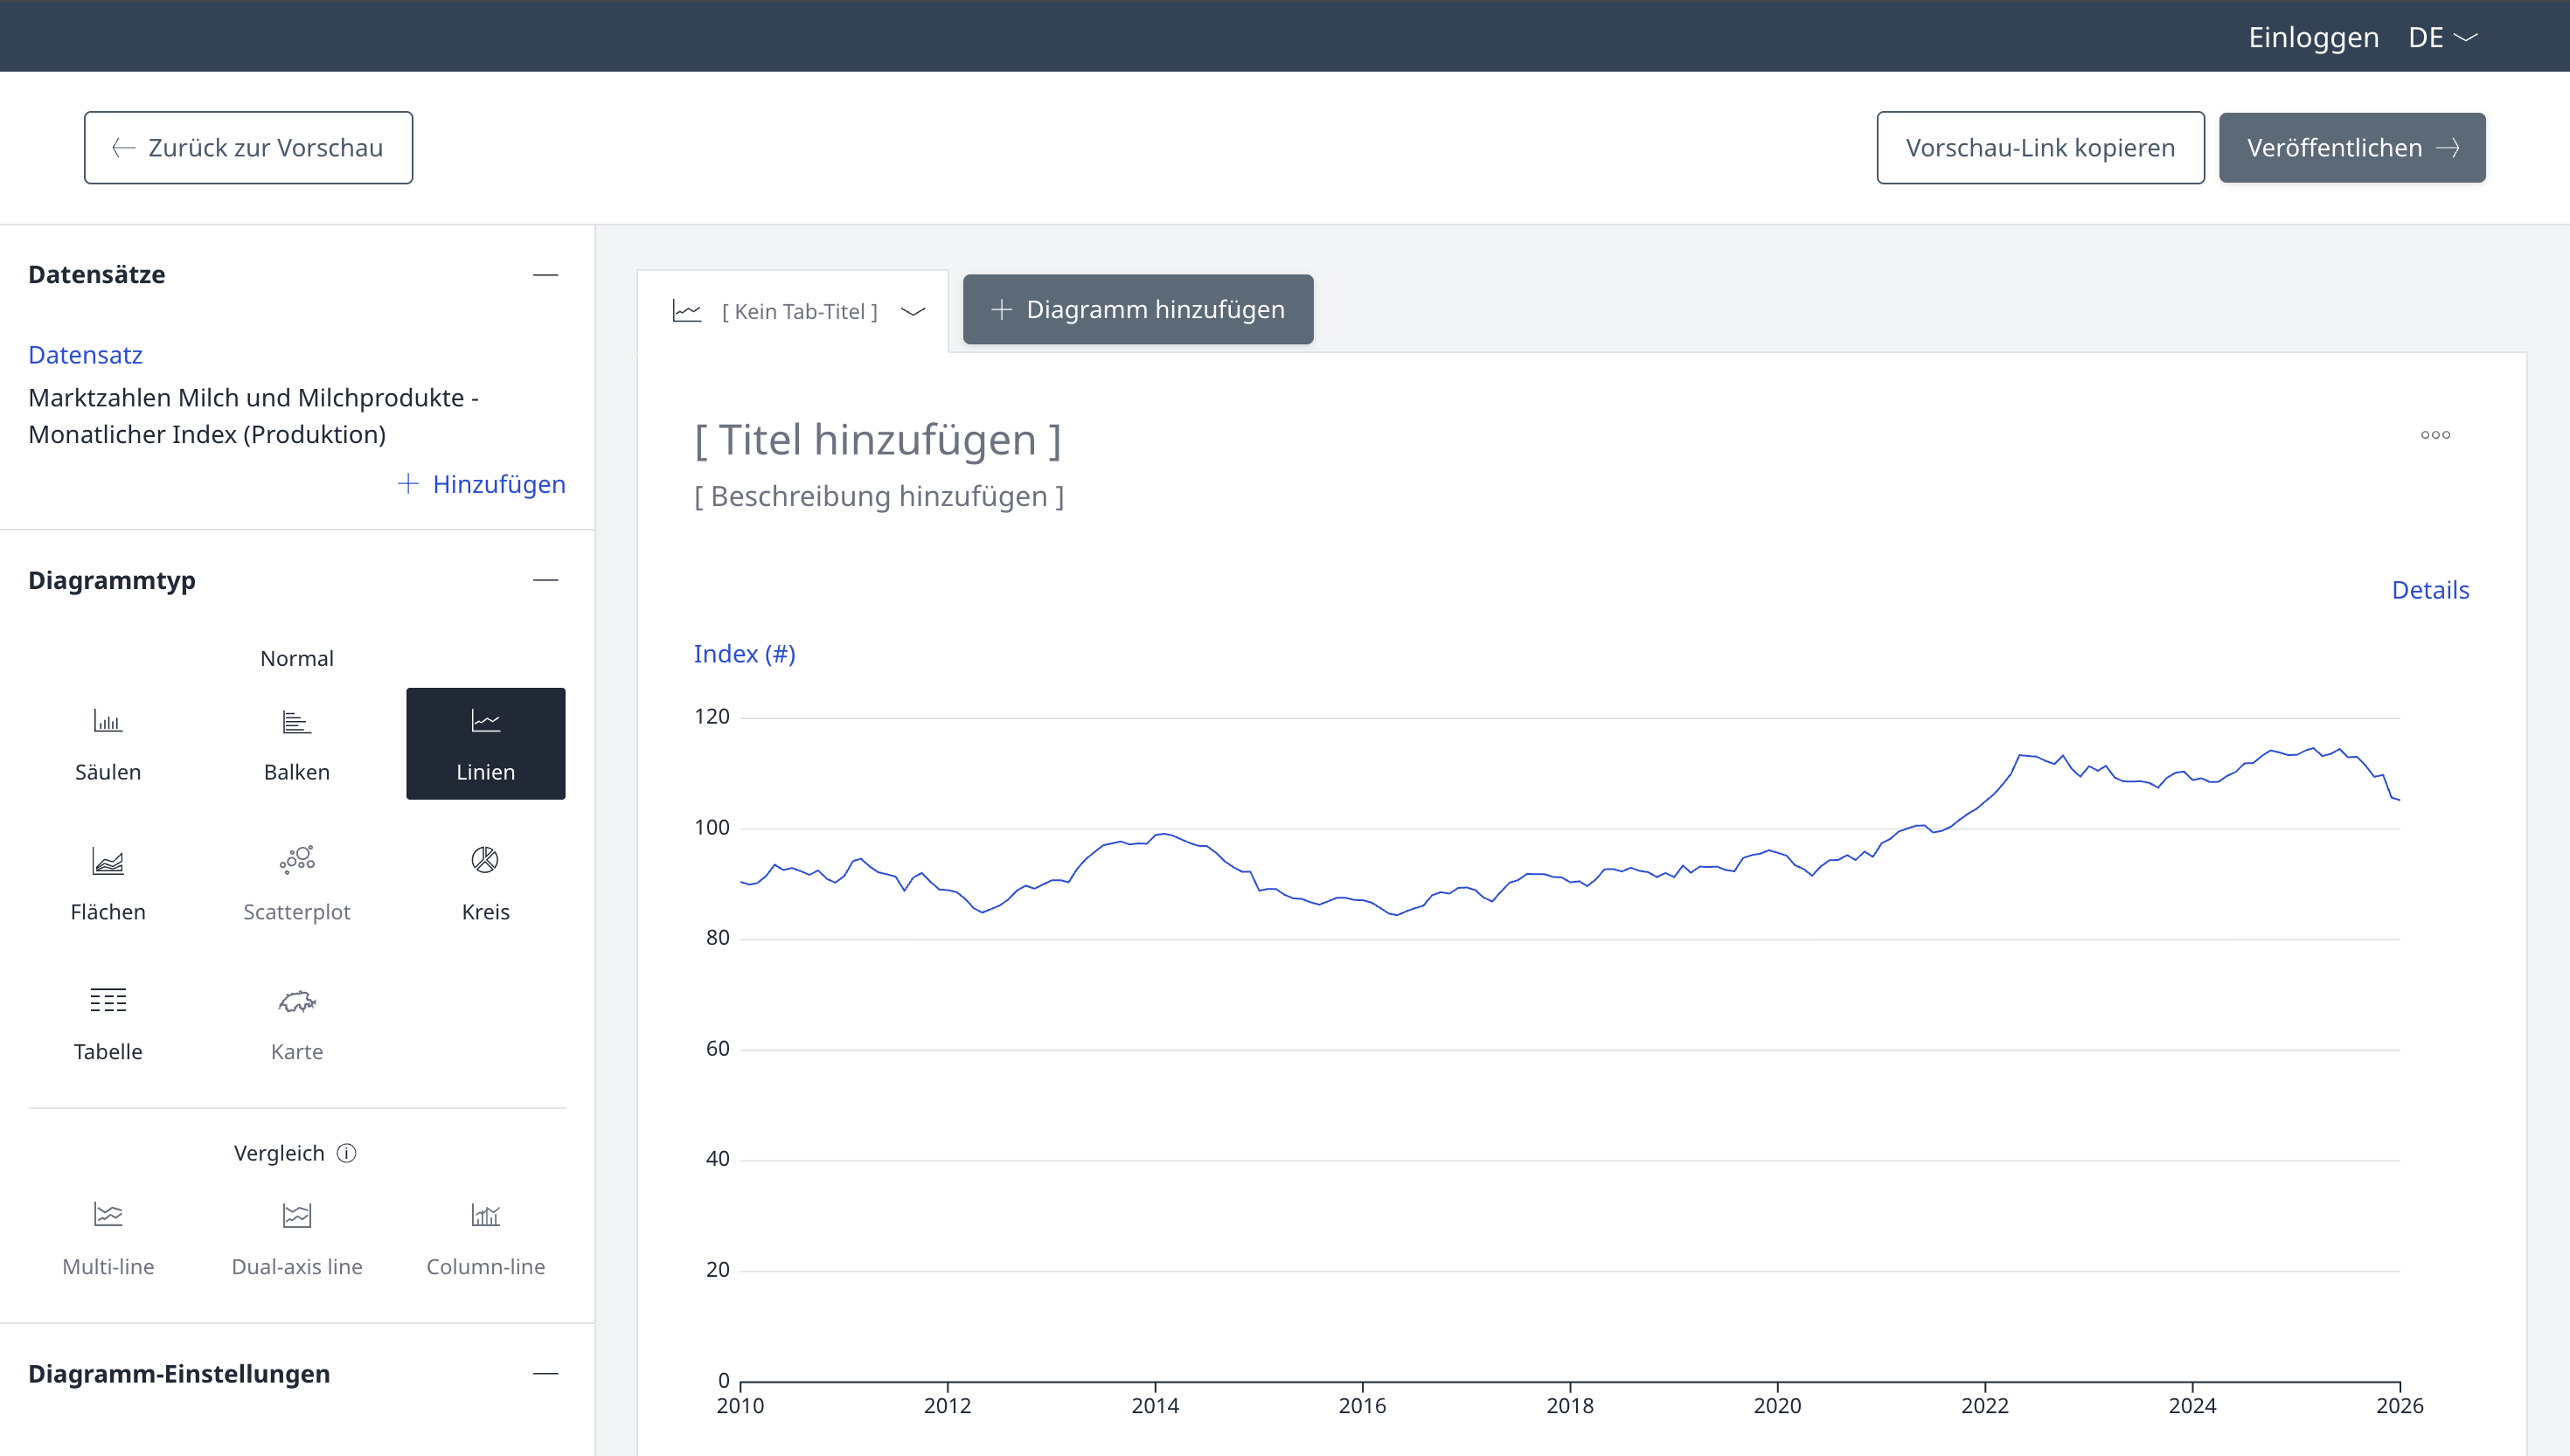
\includegraphics[width=\linewidth]{../images/SwissOpenGov_bsp.png}
        \vspace{0.4em}

        \small (b) Editor zur Erstellung eigener Visualisierungen
    \end{minipage}
    \caption{}
    \label{fig:visualize-admin}
\end{figure}

\begin{enumerate}
    \item \textbf{Vorteile}
    \begin{enumerate}
        \item Sehr fl\"ussige Bedienung auf (Außer wenn Daten geladen und verarbeitet werden).
        \item Straightforward Design.
        \item Viele Individuelle Anpassungsm\"oglichkeiten.
    \end{enumerate}

    \item \textbf{Nachteile}
    \begin{enumerate}
        \item Laiennutzung erm\"oglicht Missbrauch.
    \end{enumerate}
\end{enumerate}

\subsubsection{Eurostat}
Das Projekt Eurostat ist ebenfalls eine Open-Data-Plattform, die Datens\"atze aus der gesamten EU bereitstellt. Generell handelt es sich dabei um ein deutlich gr\"o\ss eres Projekt und um weit mehr als nur ein reines Visualisierungstool f\"ur Datens\"atze. Dennoch bietet Eurostat, wie in Bild \ref{fig:eurostat} unter (a) zu sehen ist, auch ausgew\"ahlte Datenvisualisierungen an. Diese sind, wie beispielsweise in (b) erkennbar, stets sehr ansprechend gestaltet. F\"ur ein App-Projekt w\"are eine Umsetzung in dieser Form jedoch mit einem erheblichen Aufwand verbunden. Hier muss daher der Nutzen stets gegen den erforderlichen Arbeitsaufwand abgewogen werden. Bislang bietet Eurostat jedoch die visuell ansprechendste und zugleich bestaufbereitete Darstellung von Datens\"atzen.
Vgl. \url{https://ec.europa.eu/eurostat/web/main/data/data-visualisations}

\begin{figure}[H]
    \centering
    \begin{minipage}[t]{0.48\textwidth}
        \centering
        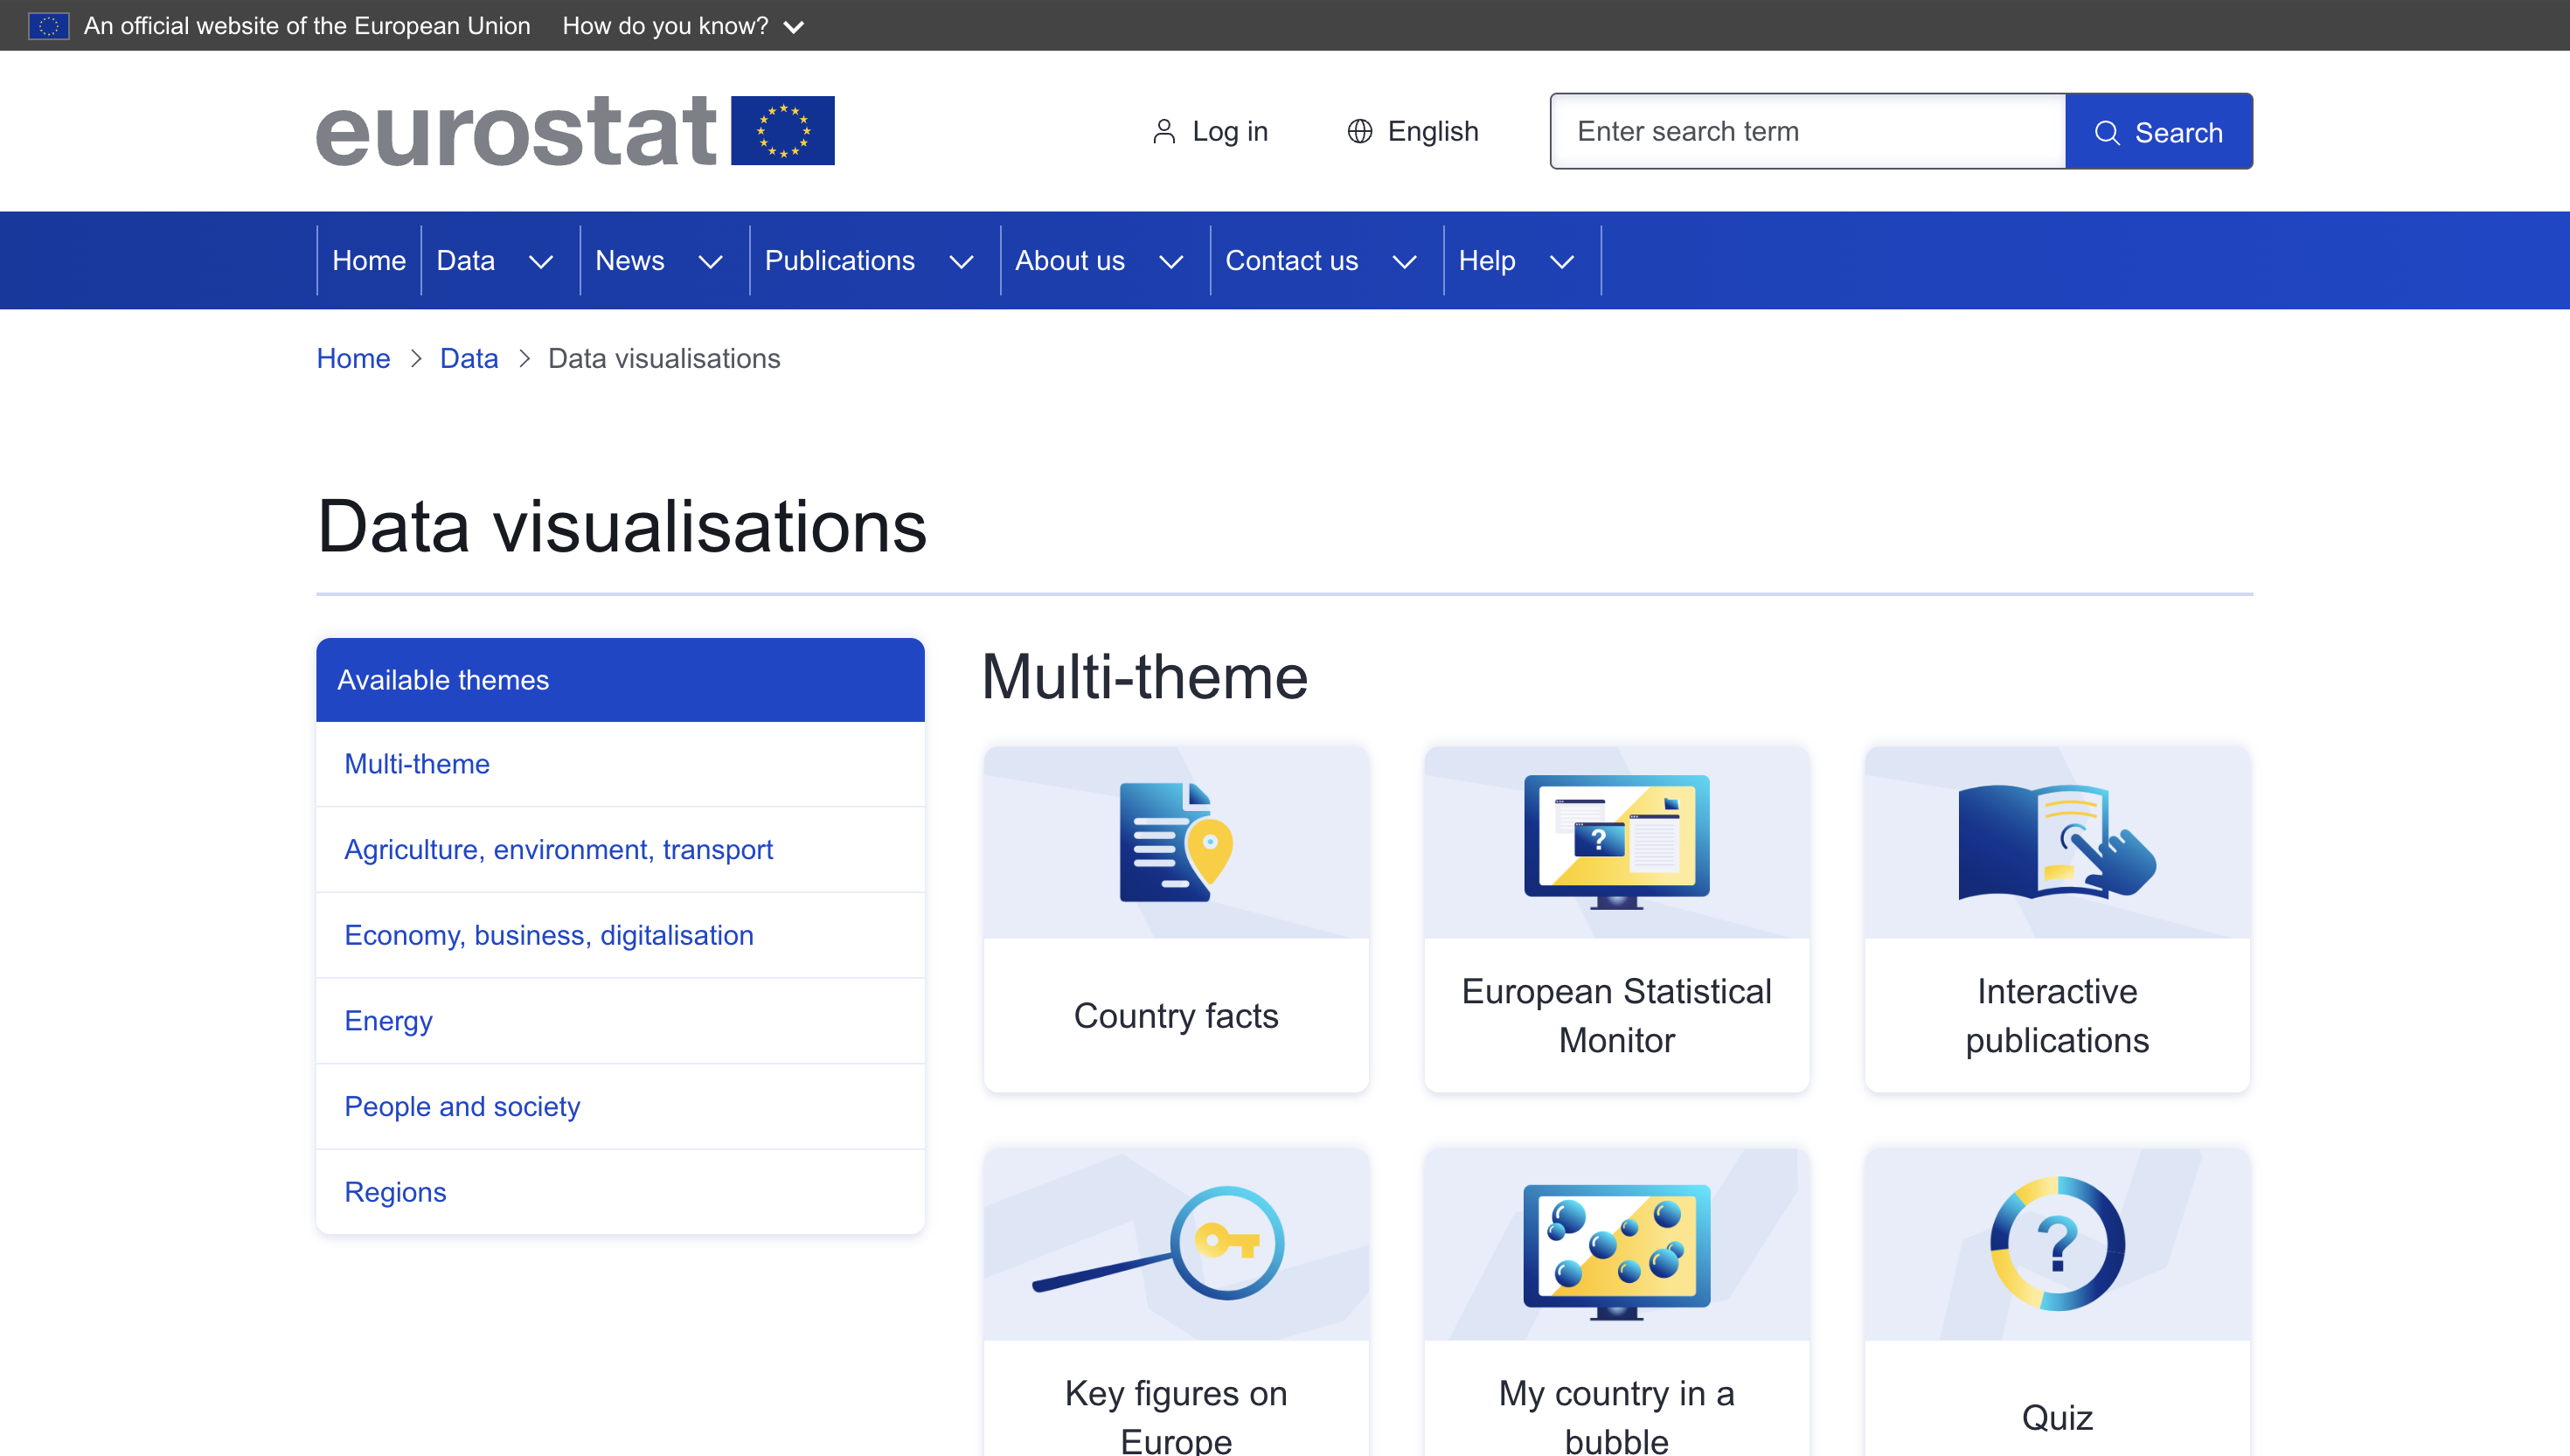
\includegraphics[width=\linewidth]{../images/EuroStat.png}
        \vspace{0.4em}

        \small (a) Übersicht der Eurostat-Datenvisualisierungen
    \end{minipage}
    \hfill
    \begin{minipage}[t]{0.48\textwidth}
        \centering
        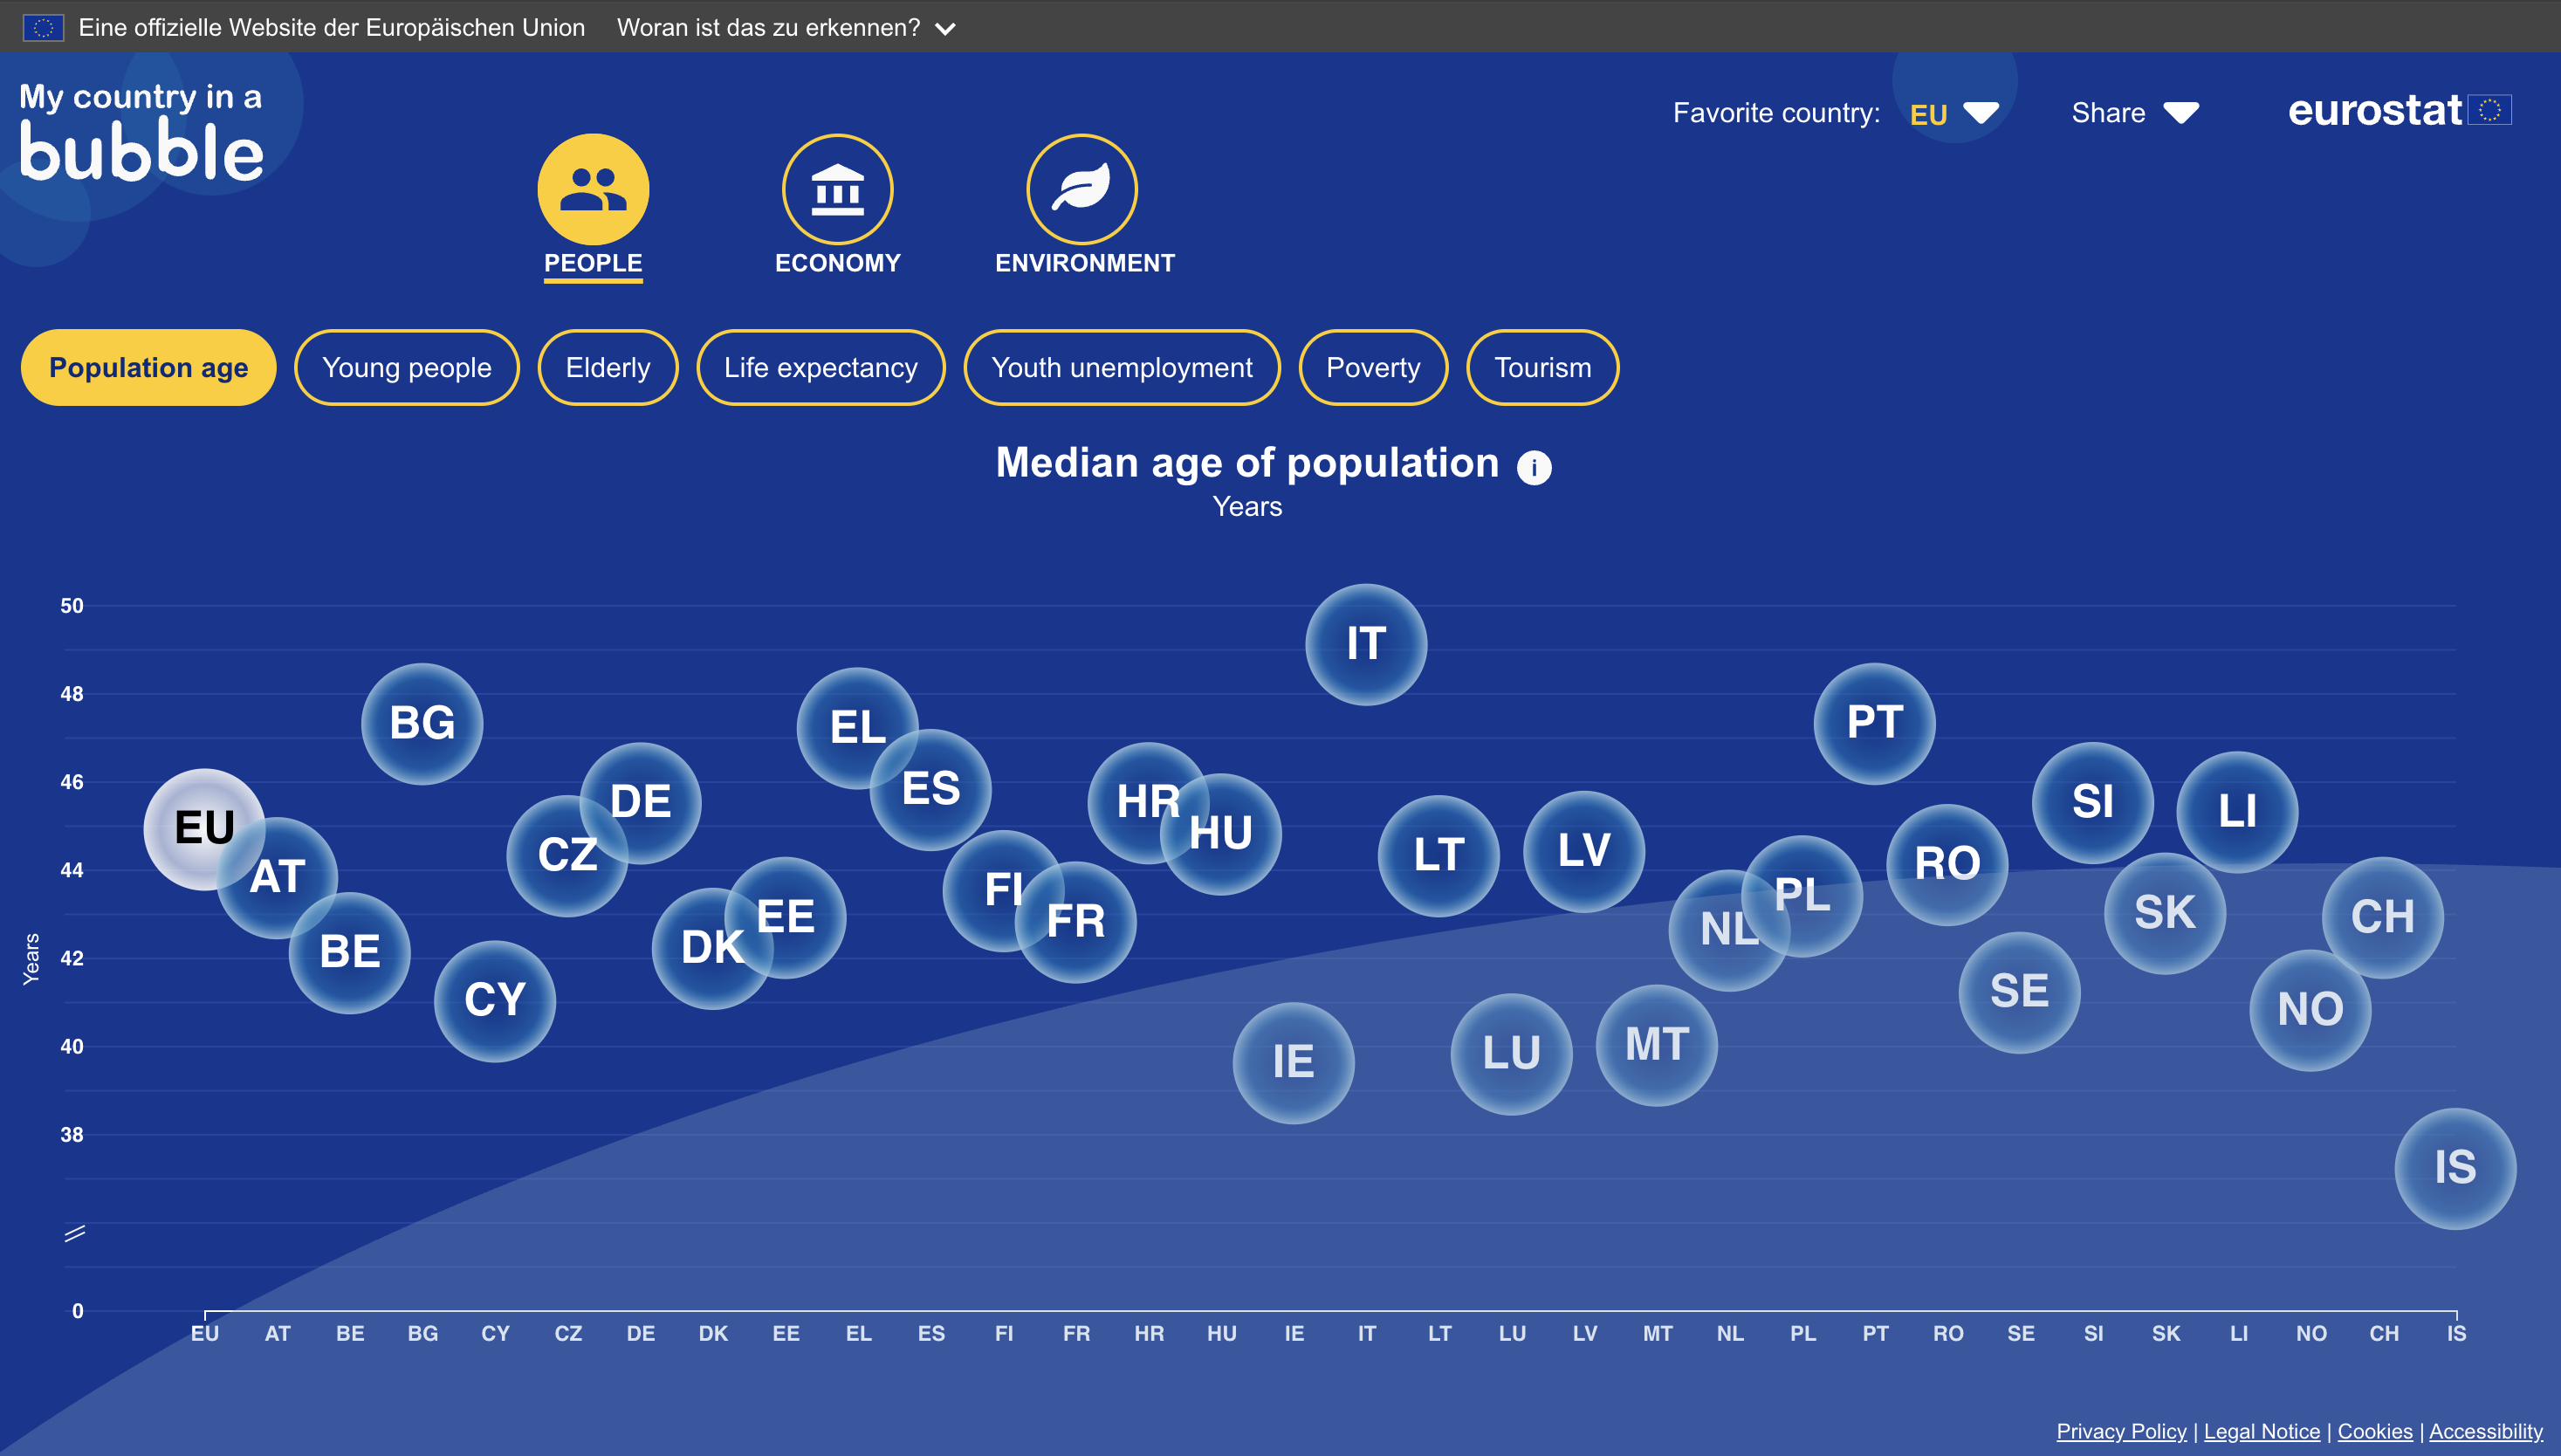
\includegraphics[width=\linewidth]{../images/EuroStat_bsp.png}
        \vspace{0.4em}

        \small (b) Interaktive Vergleichsansicht \emph{My country in a bubble}
    \end{minipage}
    \caption{}
    \label{fig:eurostat}
\end{figure}

\begin{enumerate}
    \item \textbf{Vorteile}
    \begin{enumerate}
        \item Wundersch\"one Darstellungen ausgew\"ahlter Datens\"atze.
        \item Leichte Bedienung.
    \end{enumerate}

    \item \textbf{Nachteile}
    \begin{enumerate}
        \item Wenig Individualisierbarkeit.
    \end{enumerate}
\end{enumerate}

\subsubsection{OECD Data Explorer}
Der OECD Data Explorer ist ein Angebot der OECD und fungiert sowohl als Datenbank als auch als Plattform zur Exploration von Datens\"atzen. Er erm\"oglicht es, zahlreiche Datens\"atze aus den OECD-L\"andern herunterzuladen und direkt zu visualisieren. Damit stellt er nicht nur einen Zugang zu umfangreichen Datenbest\"anden bereit, sondern bietet zugleich Werkzeuge f\"ur deren anschauliche Aufbereitung und Analyse. Vgl. \url{https://www.oecd.org/en/data/datasets/oecd-DE.html}

\begin{figure}[H]
    \centering
    \begin{minipage}[t]{0.48\textwidth}
        \centering
        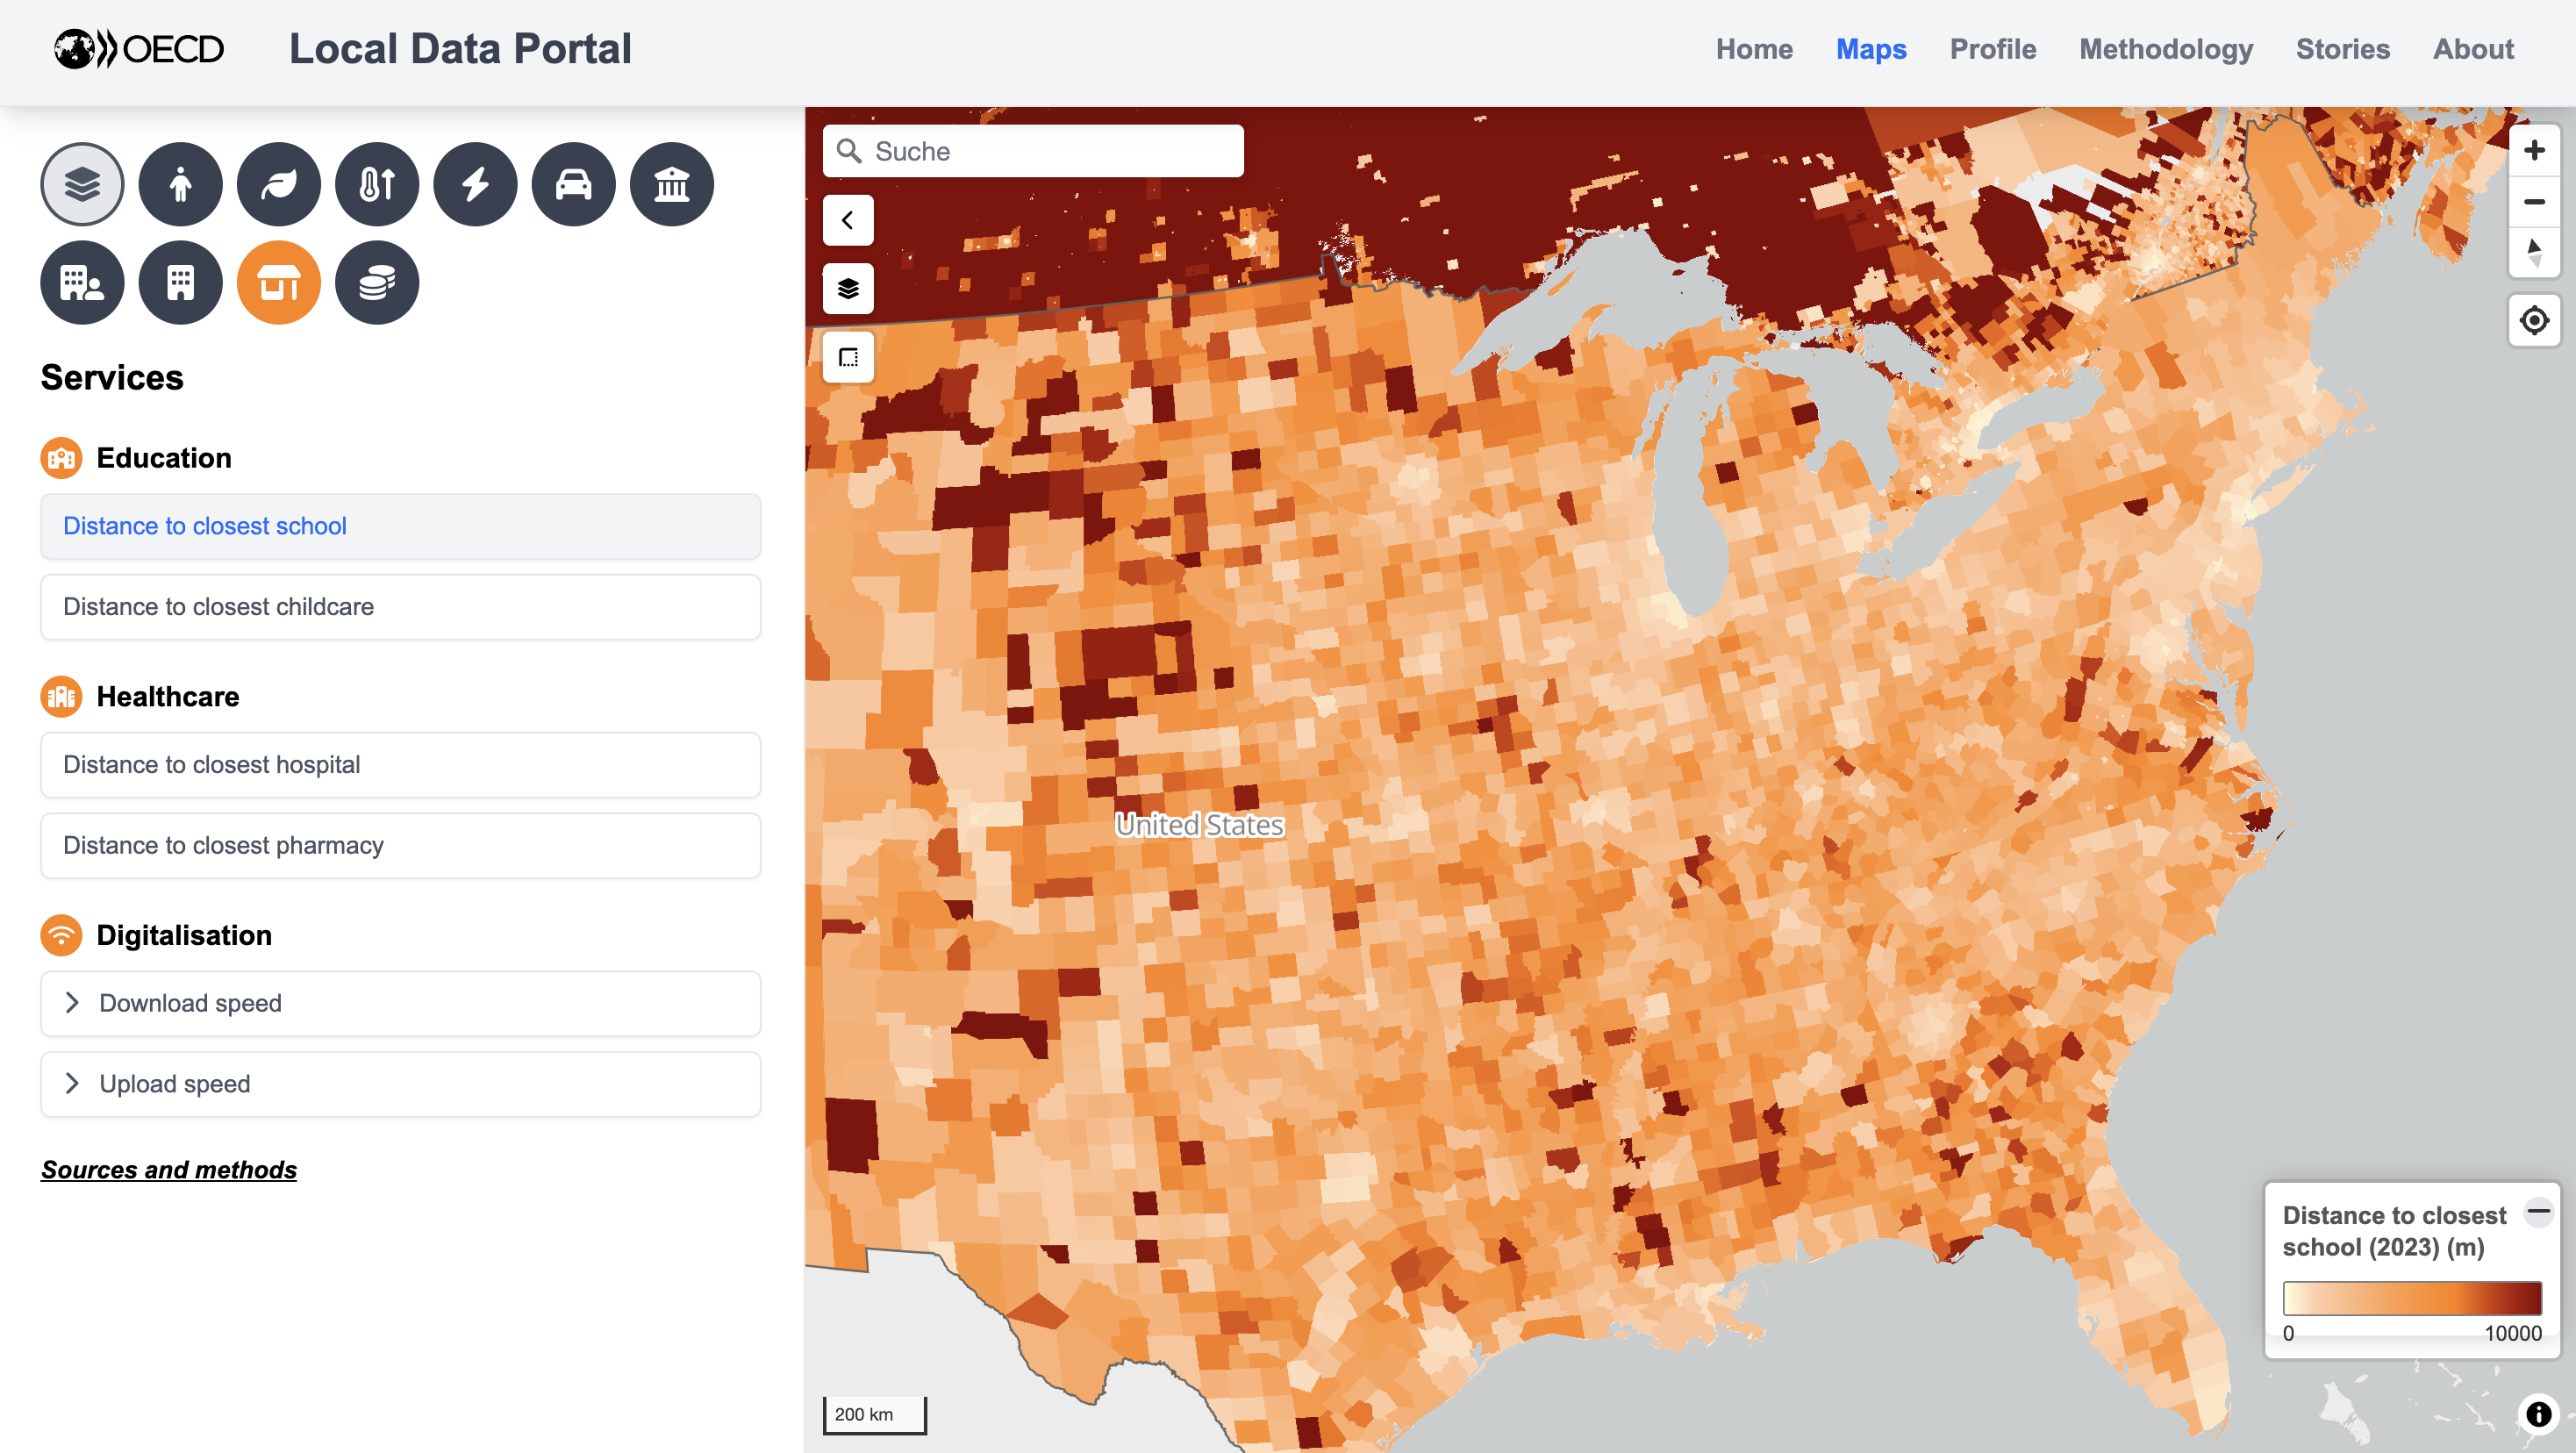
\includegraphics[width=\linewidth]{../images/OECD_Data_exp.png}
        \vspace{0.4em}

        \small (a) \emph{OECD Data Explorer} als internationales Statistikportal
    \end{minipage}
    \hfill
    \begin{minipage}[t]{0.48\textwidth}
        \centering
        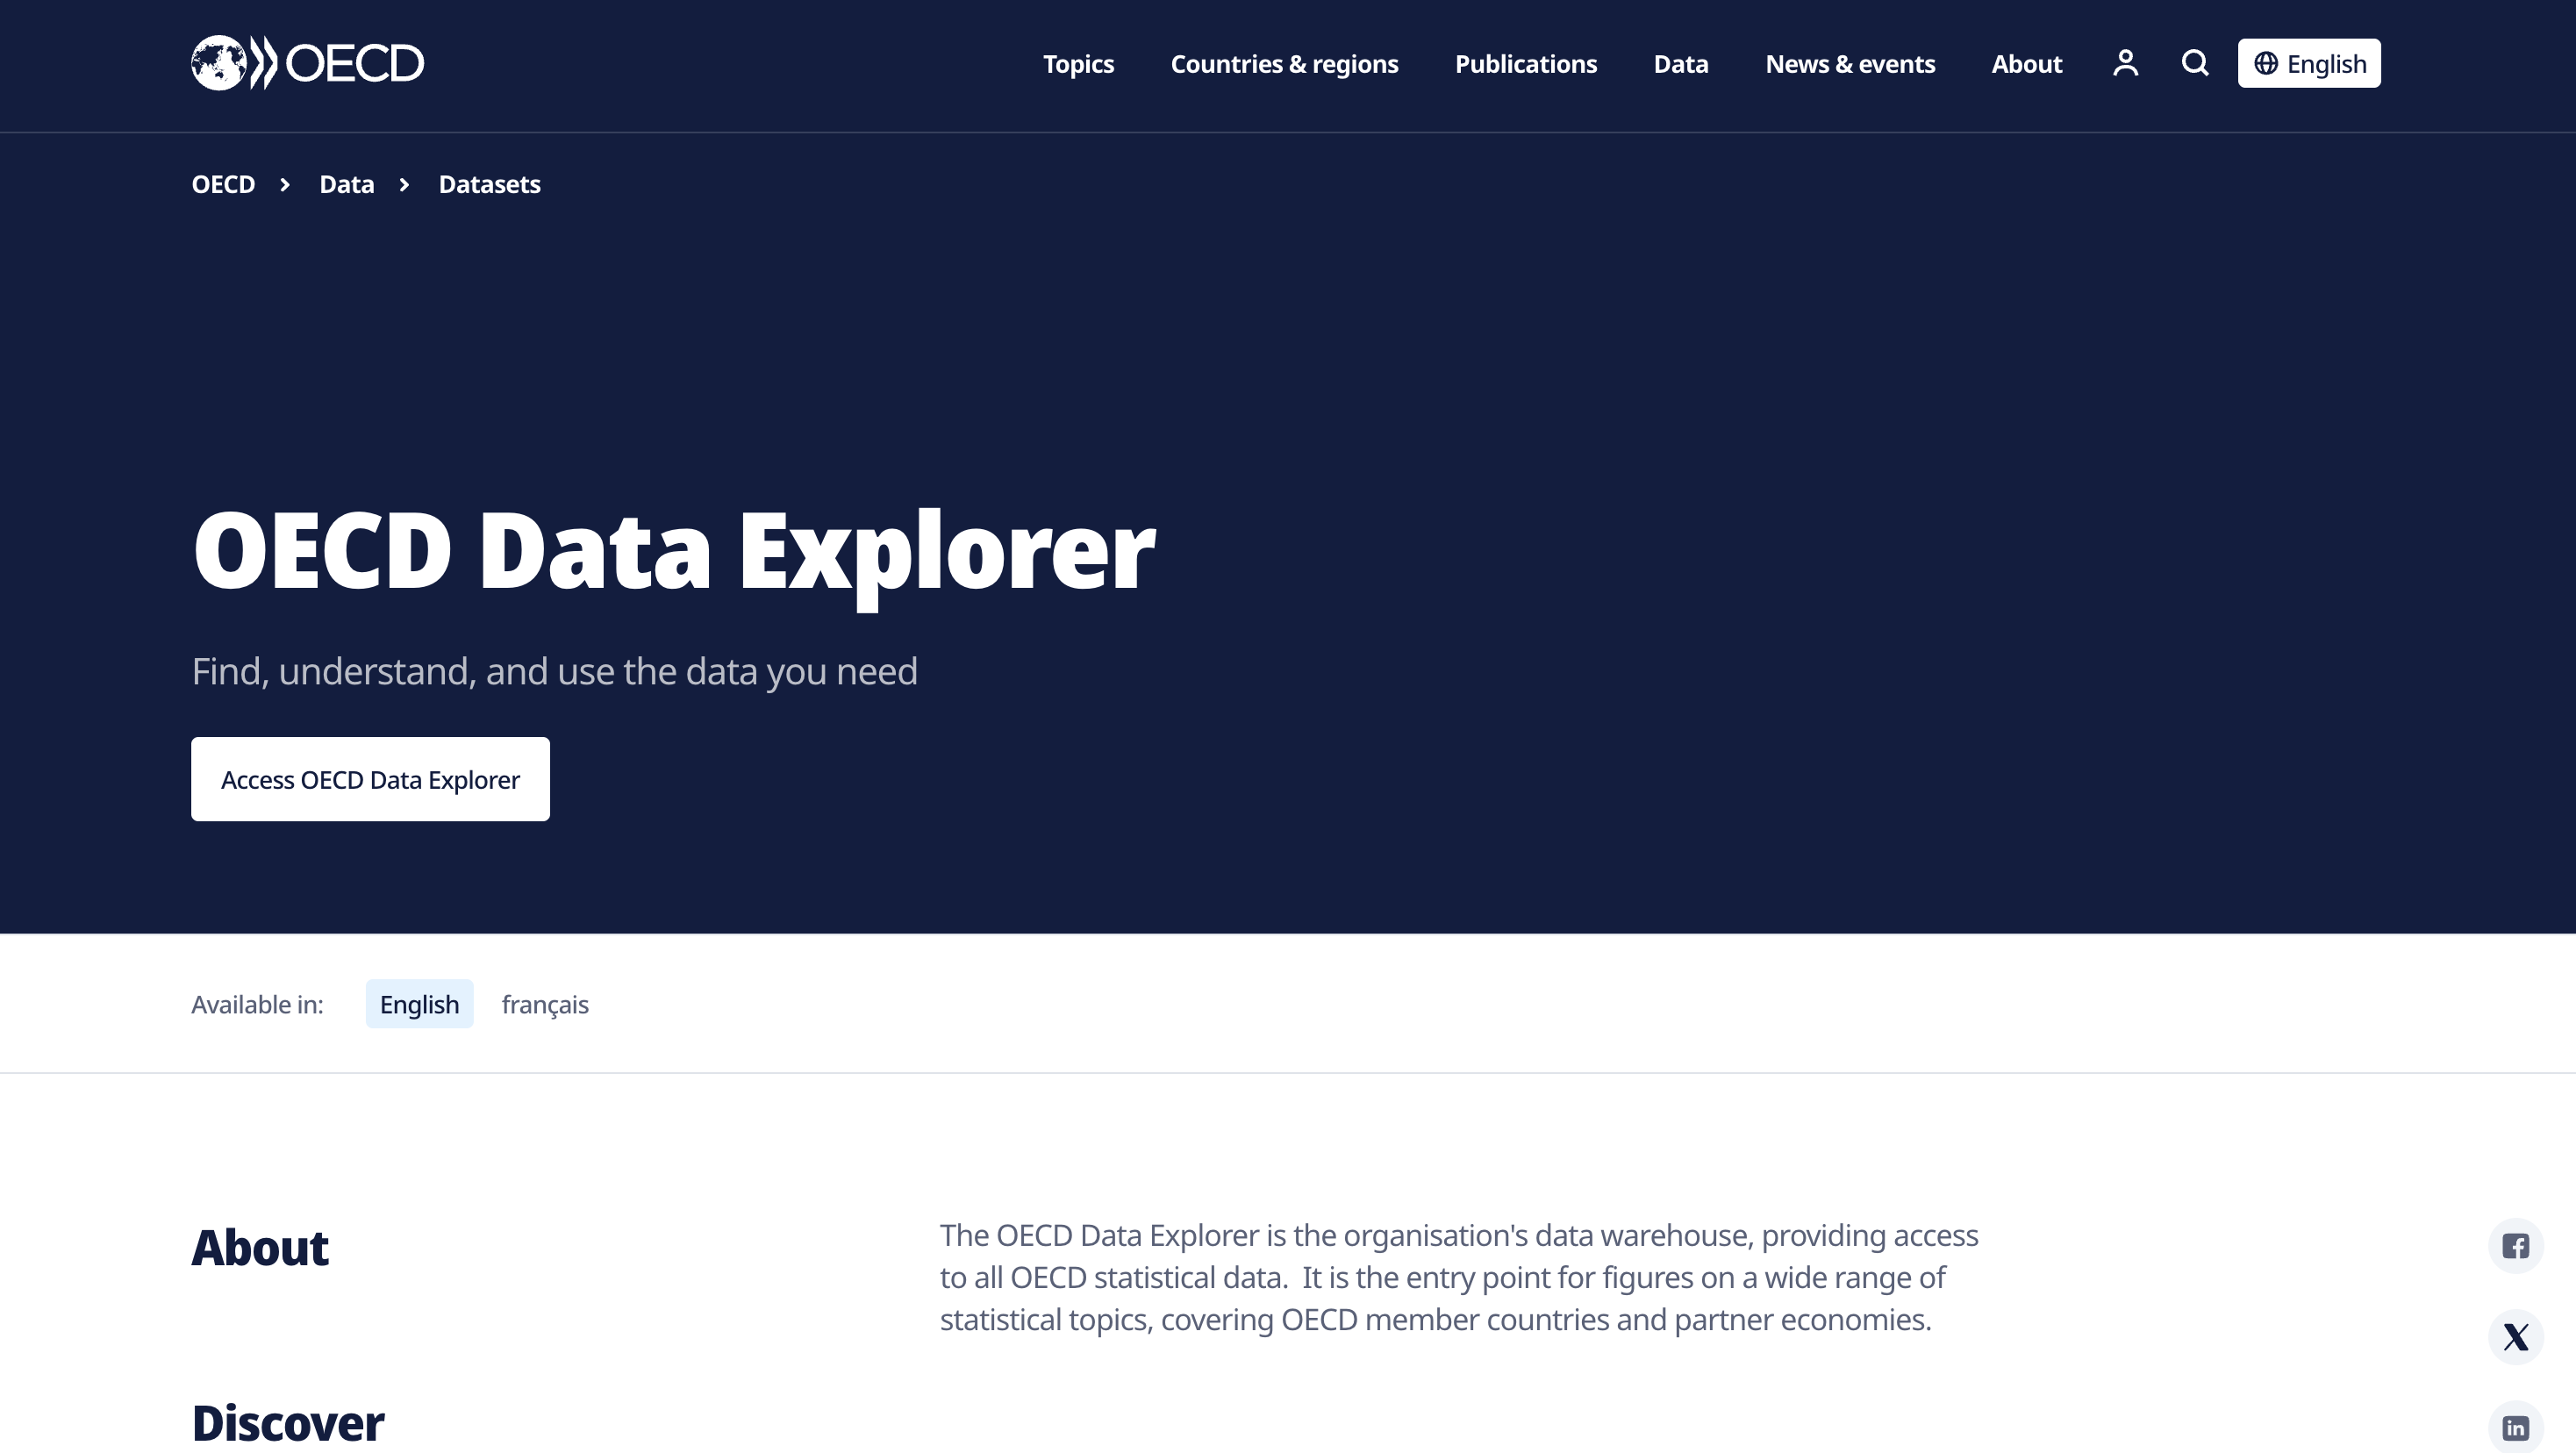
\includegraphics[width=\linewidth]{../images/OECD_DAta.png}
        \vspace{0.4em}

        \small (b) Kartenansicht des \emph{OECD Local Data Portal}
    \end{minipage}
    \caption{}
    \label{fig:oecd}
\end{figure}

\begin{enumerate}
    \item \textbf{Vorteile}
    \begin{enumerate}
        \item Große Vielfalt an Datens\"atze
    \end{enumerate}

    \item \textbf{Nachteile}
    \begin{enumerate}
        \item Schwierige und Unfl\"ussige Bedienung 
        
    \end{enumerate}
\end{enumerate}


%
\section{Nutzeranalyse und Kontextanalyse}
\lipsum[1-2]
%
\section{Erstellen Sie Personas, die die wichtigsten Nutzerszenarien abdecken}
\lipsum[1-2]
%


\section{Aufgabenanalyse}
\lipsum[1-2]
%
\section{Projektmanagement}
\lipsum[1-2]
%
\newpage
%
% Reference page, can be deleted if not used
\bibliographystyle{ieeetr}
%
\bibliography{references}
%
\end{document}